% Standalone source. Compile twice with pdfLaTeX.
% No external bibliography, figures, data, or source files are required.
\documentclass[11pt]{article}
\usepackage[T1]{fontenc}
\usepackage{lmodern}
\usepackage[margin=1in]{geometry}
\usepackage{amsmath,amssymb,amsthm}
\usepackage{booktabs}
\usepackage{tikz}
\usepackage{listings}
\usepackage{microtype}
\usepackage[hidelinks]{hyperref}
\hypersetup{pdftitle={Connected Chair-Free Graphs Without Spanning Spiders},pdfauthor={KEIO},pdfsubject={A counterexample to Conjecture 2 of Schrader and Shull}}
\newtheorem{theorem}{Theorem}
\newtheorem{lemma}[theorem]{Lemma}
\newtheorem{proposition}[theorem]{Proposition}
\newtheorem{corollary}[theorem]{Corollary}
\theoremstyle{remark}
\newtheorem{remark}[theorem]{Remark}
\newcommand{\br}{\operatorname{br}}
\newcommand{\degg}{\operatorname{deg}}
\lstset{language=Python,basicstyle=\ttfamily\footnotesize,columns=fullflexible,keepspaces=true,showstringspaces=false,breaklines=false,aboveskip=10pt,belowskip=10pt}
\setlength{\emergencystretch}{2em}
\title{Connected Chair-Free Graphs\\Without Spanning Spiders}
\author{KEIO}
\date{27 October 2026}

\begin{document}
\maketitle

\begin{abstract}
We construct a connected chair-free graph containing an induced claw but having no spanning tree with at most one branch vertex. The graph has fourteen vertices and twenty-four edges and refutes Conjecture~2 of Schrader and Shull, even when connectedness is added to its hypothesis. More generally, let $G_{p,q,k}$ consist of two anticomplete cliques of orders $p,q\geq1$, an independent set of $k\geq2$ vertices complete to both cliques, and a private pendant vertex at each clique vertex. We prove that $G_{p,q,k}$ has a spanning tree with at most one branch vertex if and only if $\min\{p,q\}\leq k$. This yields an infinite family of connected counterexamples of order $5k+4$, each requiring exactly two branch vertices. The proofs are elementary and independent of computation. An exact enumeration of all $7500$ spanning trees of the fourteen-vertex example provides a supplementary check.
\end{abstract}

\noindent\textbf{Keywords.} Chair-free graph; induced claw; spanning tree; spanning spider; branch vertex.

\section{The conjecture and the main result}

All graphs are finite, simple, and undirected. A \emph{branch vertex} of a tree is a vertex of degree at least three. A \emph{claw} is the graph $K_{1,3}$, and a \emph{chair}, also called a fork, is the five-vertex tree obtained by subdividing one edge of a claw once. A graph is chair-free, respectively claw-free, if it has no induced subgraph isomorphic to a chair, respectively a claw.

Schrader and Shull~\cite[Conjecture~2]{SS2025} proposed that every chair-free graph that is not claw-free has a spanning spider or a Hamiltonian path. In their usage, a spider has one branch vertex; allowing a Hamiltonian path is therefore equivalent to asking for a spanning tree with \emph{at most one} branch vertex. We use this combined formulation throughout. The printed conjecture does not explicitly assume connectedness. Our examples are connected, so they also refute the more restrictive connected interpretation; they do not exploit that omission.

\begin{theorem}\label{thm:main}
There exists a connected chair-free graph on fourteen vertices and twenty-four edges that contains an induced claw and has no spanning tree with at most one branch vertex. In fact, there are infinitely many such graphs, and each of the examples constructed below has a spanning tree with exactly two branch vertices.
\end{theorem}

We first give the fourteen-vertex construction and a direct proof. We then characterize exactly when a larger three-parameter family admits a spanning tree with at most one branch vertex. The final section and appendix record an independent, reproducible finite verification. No computation is used in the proofs of the counterexample or the family characterization.

\section{A fourteen-vertex counterexample}

Let $A=\{a_1,a_2,a_3\}$ and $B=\{b_1,b_2,b_3\}$ induce two disjoint triangles, with no edges between $A$ and $B$. Add two nonadjacent vertices $s,t$, each adjacent to every vertex of $A\cup B$. Finally, for each $x\in A\cup B$, add a private pendant vertex $x'$ adjacent only to $x$. Denote the resulting graph by $H_2$; see Figure~\ref{fig:h2}. We call the vertices in $A\cup B$ \emph{supports}, the vertices $s,t$ \emph{hubs}, and the vertices $x'$ \emph{private leaves}.

The graph $H_2$ is connected and has fourteen vertices and twenty-four edges. Each support has degree five, each hub has degree six, and each private leaf has degree one. For every support $x$, the set $\{x,x',s,t\}$ induces a claw centered at $x$. Thus $H_2$ is not claw-free.

\begin{figure}[htbp]
\centering
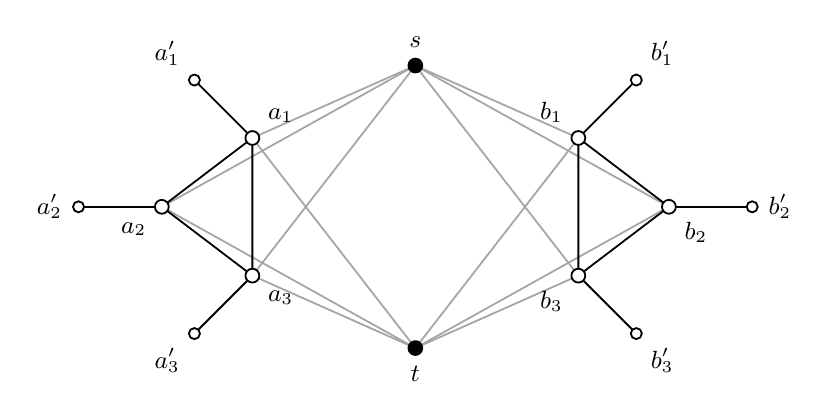
\begin{tikzpicture}[scale=.92,
  support/.style={circle,draw,fill=white,inner sep=1.6pt,minimum size=5pt},
  hub/.style={circle,draw,fill=black,inner sep=1.6pt,minimum size=5pt},
  leaf/.style={circle,draw,fill=white,inner sep=1.25pt,minimum size=4pt},
  every label/.style={font=\small},line width=.65pt]
\coordinate (a1) at (-2.25,.95);
\coordinate (a2) at (-3.5,0);
\coordinate (a3) at (-2.25,-.95);
\coordinate (b1) at (2.25,.95);
\coordinate (b2) at (3.5,0);
\coordinate (b3) at (2.25,-.95);
\coordinate (s) at (0,1.95);
\coordinate (t) at (0,-1.95);
\coordinate (ap1) at (-3.05,1.75);
\coordinate (ap2) at (-4.65,0);
\coordinate (ap3) at (-3.05,-1.75);
\coordinate (bp1) at (3.05,1.75);
\coordinate (bp2) at (4.65,0);
\coordinate (bp3) at (3.05,-1.75);
\foreach \v in {a1,a2,a3,b1,b2,b3} {
  \draw[gray!70] (s)--(\v);
  \draw[gray!70] (t)--(\v);
}
\draw (a1)--(a2)--(a3)--(a1);
\draw (b1)--(b2)--(b3)--(b1);
\foreach \i in {1,2,3} {
  \draw (a\i)--(ap\i);
  \draw (b\i)--(bp\i);
}
\node[support,label=above right:$a_1$] at (a1) {};
\node[support,label=below left:$a_2$] at (a2) {};
\node[support,label=below right:$a_3$] at (a3) {};
\node[support,label=above left:$b_1$] at (b1) {};
\node[support,label=below right:$b_2$] at (b2) {};
\node[support,label=below left:$b_3$] at (b3) {};
\node[hub,label=above:$s$] at (s) {};
\node[hub,label=below:$t$] at (t) {};
\node[leaf,label=above left:$a'_1$] at (ap1) {};
\node[leaf,label=left:$a'_2$] at (ap2) {};
\node[leaf,label=below left:$a'_3$] at (ap3) {};
\node[leaf,label=above right:$b'_1$] at (bp1) {};
\node[leaf,label=right:$b'_2$] at (bp2) {};
\node[leaf,label=below right:$b'_3$] at (bp3) {};
\end{tikzpicture}
\caption{The graph $H_2$. Each hub is adjacent to all six supports; there is no edge between the hubs or between the two triangles. Unmarked crossings are not vertices.}
\label{fig:h2}
\end{figure}

\begin{lemma}\label{lem:h2chair}
The graph $H_2$ is chair-free.
\end{lemma}
\begin{proof}
A private leaf cannot be the center of an induced claw, since its degree is one. Neither hub can be such a center: its neighborhood is the disjoint union of two triangles and contains no independent set of three vertices.

For a support $x$, its neighborhood consists of $x'$, the two hubs, and the other two vertices of its triangle. Those two triangle vertices are adjacent to each other and to both hubs. Hence the only independent triple in this neighborhood is $\{x',s,t\}$. Every induced claw is therefore one of the six claws already described.

In an induced chair, the degree-three vertex and its three neighbors induce a claw. The fifth vertex is adjacent to exactly one of those three neighbors and is nonadjacent to the claw center. A claw centered at $x$ cannot be extended in this way through $x'$, since $x'$ has no neighbor other than $x$. It cannot be extended through either hub, since $s$ and $t$ have identical neighborhoods: any vertex adjacent to one of them is adjacent to both. Therefore no induced chair exists.
\end{proof}

\begin{lemma}\label{lem:h2branch}
Every spanning tree of $H_2$ has at least two branch vertices.
\end{lemma}
\begin{proof}
Every spanning tree $T$ contains all six pendant edges $xx'$, so it has at least six leaves. For any tree on at least two vertices, the degree-sum identity gives
\begin{equation}\label{eq:leafidentity}
 L(T)=2+\sum_{\degg_T(v)\geq3}(\degg_T(v)-2),
\end{equation}
where $L(T)$ denotes its number of leaves. Indeed, subtracting twice the number of vertices from the sum of all degrees gives $-2$; vertices of degree one contribute $-1$, vertices of degree two contribute zero, and branch vertices contribute their degree minus two.

Suppose that $T$ has at most one branch vertex. A tree with no branch vertex has two leaves, so $T$ must have a unique branch vertex $r$. By~\eqref{eq:leafidentity}, $\degg_T(r)=L(T)\geq6$. Only the hubs have graph degree at least six, and both have degree exactly six. By symmetry, assume $r=s$. Then all six edges from $s$ to the supports belong to $T$.

The other hub $t$ has a tree neighbor $x\in A\cup B$. The support $x$ is incident in $T$ with $sx$, $tx$, and its forced pendant edge $xx'$. Thus $x$ is a second branch vertex, a contradiction.
\end{proof}

In particular, $H_2$ has neither a spanning spider nor a Hamiltonian path. The obstruction does not depend on choosing a particular center: Lemma~\ref{lem:h2branch} excludes every spanning tree with at most one branch vertex. The next section proves the infinite-family assertion and shows that two branch vertices always suffice for these counterexamples.

\section{An exact criterion for a three-parameter family}

For integers $p,q\geq1$ and $k\geq2$, define $G_{p,q,k}$ as follows. Let $A$ and $B$ be disjoint cliques of orders $p$ and $q$, with no edges between them. Let $S$ be an independent set of $k$ hubs, each adjacent to every support in $A\cup B$. At every support $x$, add one private leaf $x'$ adjacent only to $x$. There are no other edges. In this notation, $H_2=G_{3,3,2}$.

The graph is connected, and its order and size are
\begin{align}
 |V(G_{p,q,k})|&=2(p+q)+k,\label{eq:order}\\
 |E(G_{p,q,k})|&=\binom p2+\binom q2+(k+1)(p+q).\label{eq:size}
\end{align}
The degrees are $p+k$ on $A$, $q+k$ on $B$, $p+q$ on $S$, and one on the private leaves.

\begin{lemma}\label{lem:generalchair}
For all $p,q\geq1$ and $k\geq2$, the graph $G_{p,q,k}$ is chair-free and contains an induced claw.
\end{lemma}
\begin{proof}
As before, neither a private leaf nor a hub can be the center of an induced claw. A hub neighborhood is the union of the two cliques $A$ and $B$ and contains no independent triple.

For a support $x\in A$, the neighborhood is
\[
 N(x)=(A\setminus\{x\})\cup S\cup\{x'\}.
\]
A vertex in $A\setminus\{x\}$ is adjacent to every other vertex of that set and to every hub. Thus every independent triple in $N(x)$ lies in $S\cup\{x'\}$ and includes at least two hubs. In particular, $x'$ and any two distinct hubs form such a triple, so the graph contains an induced claw. The case $x\in B$ is identical.

Every induced chair would extend one of these claws by a vertex adjacent to exactly one claw leaf and nonadjacent to its center. A private leaf cannot be extended, because its only neighbor is the center. A hub leaf cannot be extended, because the claw has at least two hub leaves and all hubs have the same neighborhood $A\cup B$. Any vertex adjacent to one hub leaf is adjacent to another. No induced chair is possible.
\end{proof}

\begin{theorem}\label{thm:criterion}
Let $p,q\geq1$ and $k\geq2$. The graph $G_{p,q,k}$ has a spanning tree with at most one branch vertex if and only if
\[
 \min\{p,q\}\leq k.
\]
\end{theorem}
\begin{proof}
Every spanning tree contains each pendant edge $xx'$. Suppose first that $T$ is a spanning tree with at most one branch vertex. Delete all private leaves and their incident edges from $T$. The resulting graph $F$ is a tree spanning the core $A\cup B\cup S$, and
\begin{equation}\label{eq:coredegree}
 \degg_T(x)=\degg_F(x)+1\qquad(x\in A\cup B).
\end{equation}
Deleting leaves preserves connectedness on the remaining vertices and cannot create a cycle, which justifies that $F$ is a tree.

Since $k\geq2$ and the hubs are independent, the path in $F$ between two distinct hubs contains an internal support. That support has degree at least two in $F$, hence at least three in $T$. Thus $T$ has a unique branch vertex $r$, and $r$ is a support. Every other support has degree one in $F$, by~\eqref{eq:coredegree} and connectedness.

Suppose $r\in A$. Each hub $s$ must be adjacent to $r$ in $F$. Otherwise the path from $s$ to $r$ begins with a support different from $r$, making that support an internal vertex of the path, contrary to its degree being one in $F$. Since a hub is not a branch vertex, its degree in $F$ is at most two. After using its edge to $r$, each hub can therefore accommodate at most one additional support leaf.

Every vertex of $B$ is a leaf of $F$ and is nonadjacent to $r$. It cannot attach to another support different from $r$, because that support is also a leaf of $F$, and two adjacent leaves would form a component of order two in a tree with more than two vertices. It must attach to a hub. Consequently $q\leq k$. If $r\in B$, the symmetric argument gives $p\leq k$.

Conversely, suppose $q\leq k$ and choose $r\in A$. Join $r$ to all other vertices of $A$ and to every hub. Attach the $q$ vertices of $B$ to distinct hubs, one per hub. This gives a tree on the core: a star with some edges extended by one vertex. Add every pendant edge. Every support other than $r$ now has degree two, and every hub has degree at most two; the private leaves have degree one. Hence the resulting spanning tree has at most one branch vertex. The case $p\leq k$ follows by interchanging $A$ and $B$.
\end{proof}

For a connected graph $G$, define its minimum spanning-tree branch count by
\[
 \br(G)=\min_{T\text{ a spanning tree of }G}
        |\{v\in V(G):\degg_T(v)\geq3\}|.
\]

\begin{corollary}\label{cor:branchcount}
For all $p,q\geq1$ and $k\geq2$,
\[
 \br(G_{p,q,k})=
 \begin{cases}
  1,&\min\{p,q\}\leq k,\\
  2,&\min\{p,q\}>k.
 \end{cases}
\]
\end{corollary}
\begin{proof}
The path between two hubs in the core of any spanning tree has an internal support, which becomes a branch vertex after its private leaf is restored. Thus $\br(G_{p,q,k})\geq1$, and Theorem~\ref{thm:criterion} gives the first case and the lower bound in the second.

For the second case, choose $a\in A$, $b\in B$, and $s\in S$. Use the star on $A$ centered at $a$, the star on $B$ centered at $b$, the edges $as,sb$, and the edges $at$ for all $t\in S\setminus\{s\}$. These edges form a tree spanning the core. Add all pendant edges. The only branch vertices are $a$ and $b$: their degrees are $p+k$ and $q+1$, respectively, while every other vertex has degree at most two. Since $p,q>k\geq2$, both displayed degrees exceed two.
\end{proof}

\begin{corollary}\label{cor:infinite}
For every integer $k\geq2$, let $H_k=G_{k+1,k+1,k}$. Then $H_k$ is connected, chair-free, and not claw-free, and
\[
 |V(H_k)|=5k+4,\qquad
 |E(H_k)|=(k+1)(3k+2),\qquad
 \br(H_k)=2.
\]
Thus $H_k$ has neither a spanning spider nor a Hamiltonian path.
\end{corollary}
\begin{proof}
The graph properties follow from Lemma~\ref{lem:generalchair}; the order and size follow from~\eqref{eq:order}--\eqref{eq:size}. Since both clique orders equal $k+1>k$, Corollary~\ref{cor:branchcount} gives the branch count. Distinct values of $k$ give distinct orders, so the family is infinite.
\end{proof}

This completes the proof of Theorem~\ref{thm:main}. Fourteen is the smallest order in the subfamily $H_k$ with $k\geq2$; no claim is made that it is the minimum possible order of a connected counterexample. The conclusion concerns Conjecture~2, not other statements with additional hypotheses. We make no priority claim relative to other counterexamples.

\section{Exact finite verification}

The preceding arguments prove the counterexample without computation. We record a separate exhaustive check of $H_2$ for reproducibility, including its complete spanning-tree distribution.

Label the supports and hubs by
\[
 A=\{0,1,2\},\qquad B=\{3,4,5\},\qquad S=\{6,7\},
\]
and let the private leaf at support $i$ be $i+8$, for $0\leq i\leq5$. The edge set is exactly
\begin{equation}\label{eq:labelededges}
 E(H_2)=\binom A2\cup\binom B2
 \cup\bigl\{\{i,s\}:0\leq i\leq5,\ s\in\{6,7\}\bigr\}
 \cup\bigl\{\{i,i+8\}:0\leq i\leq5\bigr\}.
\end{equation}
Here $\binom X2$ denotes the set of all unordered pairs from $X$.

All $\binom{14}{5}=2002$ five-vertex subsets were checked for an induced chair, with none found. All $\binom{14}{4}=1001$ four-vertex subsets were checked for an induced claw, giving exactly six. These are precisely the claws centered at a support with its private leaf and the two hubs as leaves.

Every spanning tree contains the six pendant edges. Deleting them and the private leaves gives a bijection between spanning trees of $H_2$ and spanning trees of its eight-vertex, eighteen-edge core. The core trees are exactly the acyclic seven-edge subsets: a forest on eight vertices with seven edges is connected. An exhaustive check of all $\binom{18}{7}=31824$ candidates gives $7500$ spanning trees. After restoring the pendant edges, the branch-count distribution is as follows.

\begin{table}[htbp]
\centering
\begin{tabular}{@{}lrrrrrr@{}}
\toprule
Number of branch vertices & 0 & 1 & 2 & 3 & 4 & 5\\
\midrule
Number of spanning trees & 0 & 0 & 420 & 2952 & 3552 & 576\\
\bottomrule
\end{tabular}
\caption{Complete spanning-tree enumeration for $H_2$. No tree has more than five branch vertices.}
\label{tab:trees}
\end{table}

The total count also has an independent algebraic check.

\begin{proposition}\label{prop:treecount}
The number of spanning trees of $G_{p,q,k}$ is
\[
 \tau(G_{p,q,k})=
 k(p+k)^{p-1}(q+k)^{q-1}(p+q)^{k-1}.
\]
In particular, $\tau(H_2)=2\cdot5^2\cdot5^2\cdot6=7500$.
\end{proposition}
\begin{proof}
Forced pendant edges do not change the spanning-tree count, so it suffices to consider the core on $m=p+q+k$ vertices. On vectors supported in $A$ whose coordinates sum to zero, its Laplacian acts as multiplication by $p+k$. This gives the eigenvalue $p+k$ with multiplicity $p-1$. Similarly, the subspaces of zero-sum vectors on $B$ and on $S$ give eigenvalues $q+k$ and $p+q$ with multiplicities $q-1$ and $k-1$.

The remaining three-dimensional subspace consists of vectors constant on each of $A,B,S$. On the three block values, the Laplacian acts by
\[
 Q=\begin{pmatrix}
 k&0&-k\\
 0&k&-k\\
 -p&-q&p+q
 \end{pmatrix}.
\]
Its characteristic polynomial is $\lambda(\lambda-k)(\lambda-m)$, so the remaining eigenvalues are $0,k,m$. By the spectral form of the Matrix--Tree Theorem, the number of spanning trees of a connected graph on $m$ vertices is the product of its nonzero Laplacian eigenvalues divided by $m$. Substitution gives the stated formula.
\end{proof}

\appendix
\section{A self-contained verification program}\label{app:code}

The following program uses only the standard library of Python~3.8 or later and reconstructs the graph directly from~\eqref{eq:labelededges}. It requires no data files. Run it without \texttt{-O} so that assertions remain enabled. A five-vertex graph is a chair exactly when it is connected and has degree multiset $\{1,1,1,2,3\}$: the degree sum is eight, so connectedness makes it a tree, and its unique degree-two vertex lies on the one subdivided arm of the degree-three vertex. The four-vertex degree multiset $\{1,1,1,3\}$ characterizes a claw.

In the core enumeration, union--find rejects a candidate as soon as it creates a cycle. For a surviving candidate, the full-tree degree of a support is its core degree plus one, while the hub degrees are unchanged. The six private leaves never contribute branch vertices. The assertions check the exact counts in Table~\ref{tab:trees}; they are supplementary verification, not premises of any theorem above.

\begin{lstlisting}
from itertools import combinations
from collections import Counter
from math import comb

A, B, S = range(3), range(3, 6), (6, 7)
core = (list(combinations(A, 2))
        + list(combinations(B, 2))
        + [(v, s) for v in range(6) for s in S])
edges = core + [(v, v + 8) for v in range(6)]
adj = [set() for _ in range(14)]
for u, v in edges:
    adj[u].add(v)
    adj[v].add(u)


def connected(vertices):
    vertices = set(vertices)
    reached = {next(iter(vertices))}
    stack = list(reached)
    while stack:
        fresh = (adj[stack.pop()] & vertices) - reached
        reached.update(fresh)
        stack.extend(fresh)
    return reached == vertices


def count_induced(size, target):
    count = 0
    for vertices in combinations(range(14), size):
        part = set(vertices)
        degrees = sorted(len(adj[v] & part) for v in vertices)
        if degrees == target and connected(part):
            count += 1
    return count


chairs = count_induced(5, [1, 1, 1, 2, 3])
claws = count_induced(4, [1, 1, 1, 3])
hist, checked = Counter(), 0
for chosen in combinations(core, 7):
    checked += 1
    parent = list(range(8))
    degree = [0] * 8

    def root(v):
        while parent[v] != v:
            v = parent[v]
        return v

    for u, v in chosen:
        ru, rv = root(u), root(v)
        if ru == rv:
            break
        parent[ru] = rv
        degree[u] += 1
        degree[v] += 1
    else:
        branches = sum(degree[v] + (v < 6) >= 3
                       for v in range(8))
        hist[branches] += 1

assert len(edges) == 24 and len(core) == 18
assert comb(14, 5) == 2002 and comb(14, 4) == 1001
assert checked == comb(18, 7) == 31824
assert chairs == 0 and claws == 6
assert hist == Counter({2: 420, 3: 2952, 4: 3552, 5: 576})
assert sum(hist.values()) == 7500
print("chairs:", chairs, "claws:", claws)
print("spanning trees:", sum(hist.values()))
print("branch histogram:", dict(sorted(hist.items())))
\end{lstlisting}

\begin{thebibliography}{9}
\bibitem{SS2025}
Janee Schrader and Warren Shull,
\emph{Spanning Trees with Few Branch Vertices in a Chair-Free Graph:
Independence Number and Degree Sum Conditions},
Graphs and Combinatorics \textbf{41}, article 97 (2025).
\href{https://doi.org/10.1007/s00373-025-02945-2}{doi:10.1007/s00373-025-02945-2}.
\end{thebibliography}

\end{document}
